
% Figures in this chapter
\newcommand{\Task}{1} \newcommand{\TaskDiagram}{\Task A}
\newcommand{\TaskTrials}{\Task B} \newcommand{\TaskSounds}{\Task C}

\newcommand{\Training}{2} \newcommand{\TrainingSessions}{\Training A}
\newcommand{\TrainingTrials}{\Training B}

\newcommand{\amod}{3} \newcommand{\amodPsychometrics}{\Amod A, B, D, E}
\newcommand{\amodCorrect}{\Amod C, F}

\newcommand{\SingleSound}{4} \newcommand{\SinglePsy}{\SingleSound A, C}
\newcommand{\SingleSum}{\SingleSound B, D}
\newcommand{\SingleFreqP}{\SingleSound A}
\newcommand{\SingleFreqS}{\SingleSound B} \newcommand{\SingleAMP}{\SingleSound
C} \newcommand{\SingleAMS}{\SingleSound D}

\chapter{A behavioral task for evaluating the cortical and subcortical
contributions to sound feature discrimination}

\section{Introduction}
% We found that corticostriatal and thalamostriatal pathways send different
% information about certain sound features to the striatum.  TODO: Chapter
% number
In the last chapter, we found that the thalamostriatal and corticostriatal
pathways send complementary information to the striatum about some features of
sound. 
%
While both pathways conveyed frequency information to the striatum with similar
fidelity, corticostriatal neurons better represented the rate of temporal
amplitude modulations in their overall spiking rate.
%
The spiking rate of thalamostriatal neurons more closely followed rapid
variations in stimulus amplitude, but the total number of spikes during the
stimulus was less indicative of the modulation rate.
% What is the significance of this difference?  TODO: Chapter number
While our earlier experiments in Chapter 2 strongly suggested a role for the
striatal target region of these projections in sound-guided behavior, the
relative contribution of these parallel pathways to behavior is unclear. 
%

% Some inactivation studies show that AM discrimination suffers after cortical
% lesions.
Lesion studies have suggested that discrimination of fast AM rates suffers
following removal of auditory cortex \citep{Deutscher2006}.
%
In contrast, sound frequency discrimination behavior has been shown to persist
after extensive lesions of AC \citep{Gimenez2015}.
%
% TODO: Phrase as either/or? or cortical/subcortical?
We therefore hypothesized that the cortical representation of AM is necessary
for accurate AM discrimination, but that sound frequency discrimination can be
accomplished with auditory information from the subcortex alone. 

% Specific hypothesis and test
Specifically, we hypothesized that the effect of reversible AC inactivation
would be greater on AM discrimination than on frequency discrimination. 
%
To test this hypothesis, we designed and implemented a behavioral task that
permits evaluation of the effects of a single reversible inactivation on
discriminations of both sound features.
%
We performed bilateral reversible inactivations of AC in animals trained on
this task, and found that discrimination of both features was impaired. 
%
While the contribution of the thalamostriatal and corticostriatal pathways to
discrimination of these sound features is still not clear, this task provides a
method for comparing the effect of reversible chemical manipulations on
discriminations of diverse stimulus features. 


\section{Methods}

\subsection{Animal subjects}
% DONE: Number of mice
14 adult male wild-type mice (C57/BL6J) were used in this study. Mice had ad
libitum access to food, but water was restricted. Free water was provided on
days with no experimental sessions. All procedures were carried out in
accordance with National Institutes of Health standards and were approved by
the University of Oregon Institutional Animal Care and Use Committee.

\subsection{Behavioral task}
% DONE: Update methods for amod task
Behavioral data was collected using the taskontrol platform
(\url{www.github.com/sjara/taskontrol}) developed in our laboratory using the
Python programming language (\url{www.python.org}).
%
Mice initiated each trial by poking their noses into the center port of a
three-port behavior chamber.
%
% DONE: We aren't making animals wait - check the paradigm After a silent delay
% of random duration (150-250 ms, uniformly distributed), a sound was presented
% for 500 ms.
%
The sound was either a narrow-band sound (chord), a single tone, or a
sinusoidally-amplitude-modulated white noise.
%
The decision to use chords or tones was chosen by the experimenter, and
thereafter during the behavior session the type of stimulus alternated between
cords/tones and AM sounds each trial (stimulus type was not randomized per
trial).
%
Animals were required to stay in the center port until the end of the sound and
then chose one of the two side ports for reward (2 $\mu$l of water) according
to a reward contingency that was specific to the type of sound.
%
For chords and tones, the reward contingency was: low frequency: go to left
port; high frequency: go to right port.
%
For amplitude-modulated noise, the reward contingency was: slow modulation
rate: go to left port; fast modulation rate: go to right port.
%
If animals withdrew before the end of the stimulus, the trial was aborted and
ignored in the analysis.
%
Chord stimuli were 12 simultaneous pure tones logarithmically spaced in the
range f/1.2 to 1.2f for a given center frequency f.
%
Within a behavioral session, we used 8 distinct center frequencies for chords
and tones, and 8 distinct modulation rates for AM sounds.
%
Each behavioral session lasted 60 to 90 minutes.

\subsection{Muscimol inactivation}
% TODO: Change to match muscimol protocol for amod study. 
Bilateral craniotomies were performed under stereotactic surgery over the
posterior striatum (1.7 mm posterior to bregma, 3.55 mm lateral from midline)
of mice trained in the two-alternative choice sound discrimination task.
Headbars were implanted to allow for head-fixation. Each craniotomy was
protected with a plastic ring and filled with silicon elastomer (Sylgard 170,
Dow Corning). Animals were allowed to recover for at least 3 days before
resuming behavioral training. Following recovery, implanted animals were
trained on the sound discrimination task until they reached their pre-surgery
performance level before beginning muscimol inactivation.

For intracranial injection, we used glass pipettes (5 $\mu$l Disposable
Micropipettes, VWR) pulled and trimmed to an inner diameter of 15-20
micrometers at the tip. Animals were head-fixed and allowed to run on a wheel
during the injection. Craniotomies were exposed by removing the silicon
elastomer covering, and a glass pipette filled with reagent (either muscimol or
saline) was lowered into the brain to a depth of 3.1mm from brain surface using
a micromanipulator. A volume of 45 nl of muscimol (0.25 mg ml$^{-1}$, final
dose of 11.25 ng per hemisphere) was injected under air pressure in each
hemisphere at a rate of 90 nl min$^{-1}$.
%
% Given the relationship between concentration and diffusion distance (from
% Fick's law) and previous reports of muscimol effects on neuronal activity
% \citep{Edeline2002}, we expect that by the first 10 minutes of the behavioral
% session, the effects of muscimol (50\% reduction in firing or more) will be
% confined to a volume smaller than 1 mm in diameter centered at the injection
% site. This volume matches well the extent of the posterior tail of the
% striatum (approx. 1 mm A-P, 0.6 mm M-L, 1.5 mm D-V) that receives auditory
% inputs \citep{Hunnicutt2016}.
%
The pipette was left in place for 60 seconds following the injection, then
raised 0.5mm and left in place for another 60 seconds before being removed.
Injection in the second hemisphere was always completed within 10 minutes of
the first injection. The craniotomies were then protected with a new silicon
elastomer cap, and the mouse was placed back into its home cage for 30 minutes
before starting the behavior session. After collection of 4 saline sessions and
4 muscimol sessions, 45 nl of fluorescent dye (DiI, Thermo Fisher Scientific)
was injected at the same injection coordinates. Animals were then perfused
transcardially with 5\% paraformaldehyde, and brains were extracted and
postfixed for 12-24 hours. Brains were then sliced (100 um) and imaged to
verify the location of fluorescent dye injection.

\subsection{Analysis of behavioral data}

% DONE: Add stuff about the GLMER models here.
Psychometric curve fitting was performed via constrained maximum likelihood to
estimate the parameters of a logistic sigmoid function
(\url{http://psignifit.sourceforge.net}). Statistical comparisons were
performed using non-parametric statistical tests with no assumption of
normality. 
%
Generalized linear mixed models were fit with the R programming language
(\url{https://www.r-project.org/}) using the `lme4' package
(\url{http://lme4.r-forge.r-project.org/}).


\section{Results}

% TODO: Table number
We found that this task was challenging to learn, but that animals could learn
to perform it well if given sufficient training time.
%
We used a set of criteria defined in Table 1 to determine when mice were ready
to advance to the next training step.
%
Animals first advanced through a series of behavioral stages designed to
familiarize them with the behavior box and begin to teach them the rules of the
task.
%
During the first stage, animals received a water reward after poking their nose
in any of the three ports in the box.
%
This stage allowed animals to learn that the behavior box is a good place to
be, and engaged their natural desire to explore to teach them that they are
able to control the environment and trigger changes by poking in the ports.
%
% TODO: Make sure I am doing this right!
In the next stage, animals had to poke in the center port and then go to the
side ports to collect water.
%
This stage began to teach the animals that the center port is where you go to
trigger trials, and that going to a side port is how you collect reward.
%
After this stage, animals began to learn the sound-action association.
%
% TODO: Mention sound above
During the next stage, animals triggered a trial by poking in the center port,
and then had to go to the right port to collect a reward if the AM rate of the
presented sound was fast, and to the left port if the AM rate was slow.
%
However, on this stage animals were guided towards forming the correct
association by letting them correct their choice if they first made a mistake.
%

After animals performed well on this stage, we started requiring animals to
make a correct choice on the first try.
%
% TODO: define the range
When they were performing well on this stage, we began presenting a range of AM
rates between the previously-trained fast and slow rates.
%
During this stage, animals had to learn the category boundary between the
``fast'' and ``slow'' rates.
%
Once they became proficient at this discrimination, animals had good knowledge
of the task structure and rules.
%
At this point, we began to train on two narrow-band stimuli (or pure tones for
some animals).
%
We then switched to a stage where we presented a range of tonal stimuli, and
trained animals until they had learned the boundary between ``high'' and
``low'' sound frequencies as well.
%
% TODO: At this point is ambiguous does it mean this or the next one?
At this point we started to introduce the next level of task complexity.

During the next training stage, the type of sound presented when animals
triggered a trial switched between an AM noise and a narrow-band chord (or pure
tone) every other trial.
%
% TODO: Takes little time to do, which is a cool feature. Talk about that here. 
The sound-action association necessary to receive reward was the same as had
been previously learned for each sound.
%
We first introduced animals to the type of sound switching by presenting only
two examples of each sound type, but then moved on to presenting a range of AM
rates and sound frequencies.
% TODO: From here start to talk about performance on the psychometric version
% of full task.
%%%%%%%%%%% Training structure table %%%%%%%%%%%%%%

%% \begin{table}[]
%% \begin{tabular}{lllll}
%% \textbf{Stage} & \textbf{Name}       & \textbf{Goal}                              & \textbf{Water delivery}                                       & \textbf{Criterion to advance}              \\
%% SD AM          & Sides Direct, AM    & Get animals to poke and collect water      & After center or side poke                                     & One session with 200 rewards               \\
%% D AM           & Direct, AM          & Trial initiation in center poke            & After center poke                                             & One session with 200 rewards               \\
%% NC AM          & On next correct, AM & Train animal on correct association        & After correct side poke (OK if incorrect poke was made first) & One session with 500 rewards               \\
%% IC AM          & If correct, AM      & Require animal to make correct association & After correct side poke                                       & Animal performs \textgreater{}80\% correct
%% \end{tabular}
%% \end{table}

%%%%%%%%%%%%%%%%%%%%%%%%%%%%%%%%%%%%%%%%%%%%%%%%%%%


\subsection{Animals can switch between discriminations of different stimulus
features every trial}

Despite the difficulty of learning this task, which was evident by the long
time required for animals to progress through all of the many training stages,
animals were able to achieve high levels of performance.
% TODO: I need a figure with some psychometrics showing good performance. 

%%%%%%%%%%%%%%%%%%%%%%%% Figure Task %%%%%%%%%%%%%%%%%%%%%%%%%%%%%
\begin{figure}[hp] \begin{center}
	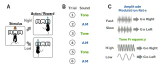
\includegraphics[width=6in]{figures/chapter4/figure_task} \end{center}
	\caption{A behavioral task for evaluating the effects of reversible
	inactivation on discrimination of different sound
	features.}{\textbf{(A)} Schematic of the two-alternative choice sound
	feature discrimination task. Mice initiated each trial by entering a
	center port and had to choose one of two side reward ports depending on
	the sound presented.
	%
\textbf{(B)} The type of sound presented was alternated every other trial. 
%
% TODO: Make sure all other figure captions have bolded cap. labels
\textbf{(C)} On trials when an AM noise stimulus was presented, mice had to
choose the right reward port if the modulation rate was fast and the left
reward port if the modulation rate was slow to be rewarded. On trials when a
narrow band chord was presented, mice were rewarded for picking the right port
if the sound frequency was high and the left port if the sound frequency was
low. 
%
}
\end{figure}
%%%%%%%%%%%%%%%%%%%%%%%%%%%%%%%%%%%%%%%%%%%%%%%%%%%%%%%%%%%%%%%%%%%%%

% TODO: I think this figure should come earlier. 
%%%%%%%%%%%%%%%%%%%%%%%% Figure Training Time %%%%%%%%%%%%%%%%%%%%%%%%%%%%%
\begin{figure}[hp] \begin{center}
	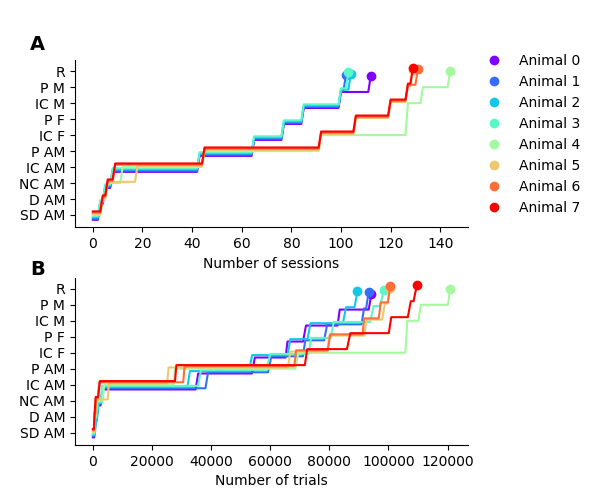
\includegraphics[width=6in]{figures/chapter4/figure_training}%
\end{center} \caption{Animals took about 4 months to learn the
task.}{\textbf{(A)} Animals progressed through 9 training steps over an average
of 119 behavioral training sessions before being ready for experiments (min:
102 sessions; max: 144 sessions). 
%
\textbf{(B)} Animals performed aN average of 100,892 trials before being ready
for experiments (min: 89,527; max: 120,885). 
%
} \end{figure}
%%%%%%%%%%%%%%%%%%%%%%%%%%%%%%%%%%%%%%%%%%%%%%%%%%%%%%%%%%%%%%%%%%%%%

\subsection{Reversible inactivation of AC affects discrimination of both sound
frequency and AM rate} After animals had learned the task, we began performing
bilateral intracranial injections of either the GABA agonist muscimol, or a
saline control, 30 minutes before each behavioral sessions.
%
We alternated between muscimol and saline injections each day. 
%
Muscimol injection affected performance on both tone and AM trials, resulting
in both a flattening of the psychometric curve (\fig{\amodPsychometrics}) and a
reduction in overall performance (\fig{\amodCorrect}) for both animals tested. 
%
We tested the hypothesis that muscimol has a stronger effect on AM
discrimination performance than on frequency dicrimination performance by
comparing two generalized linear mixed effect regression models, both attempting
to explain the variance in correct response liklihood that was explained by the
identity of the bolus. 
%
In the null model, we allowed the intercept to differ between data from the two
sound types.
%
This inclusion of a random intercept for different sound types was
well-justified from the fact that animals oftern performed much better on the
frequency discrimination trials than on AM discrimination trials.
%
Aganist this null model we compared a model which allowed both random
intercept for sound type, allowing for the fact that performance started
at a different level, as well as allowing for random slopes (a difference in
the strength of the effect beteween the two sound types).
%
For both models we additionally allowed the slope and intercept of the muscimol
effect to vary between the animals included in the comparison (n=2). 
%
Allowing for random slopes of the effect of muscimol based on sound type did
not significantly increase the variance explained by the model
($\chi^{2}$=1.64, p=0.44).
%
Therefore, we fail to reject the null hypothesis that the strength of the
muscimol effect is the same for discrimination of frequency and AM rate. 

% Inactivation caused deficits in discrimination of both types of stimuli.
\begin{figure}[hp] \begin{center}
	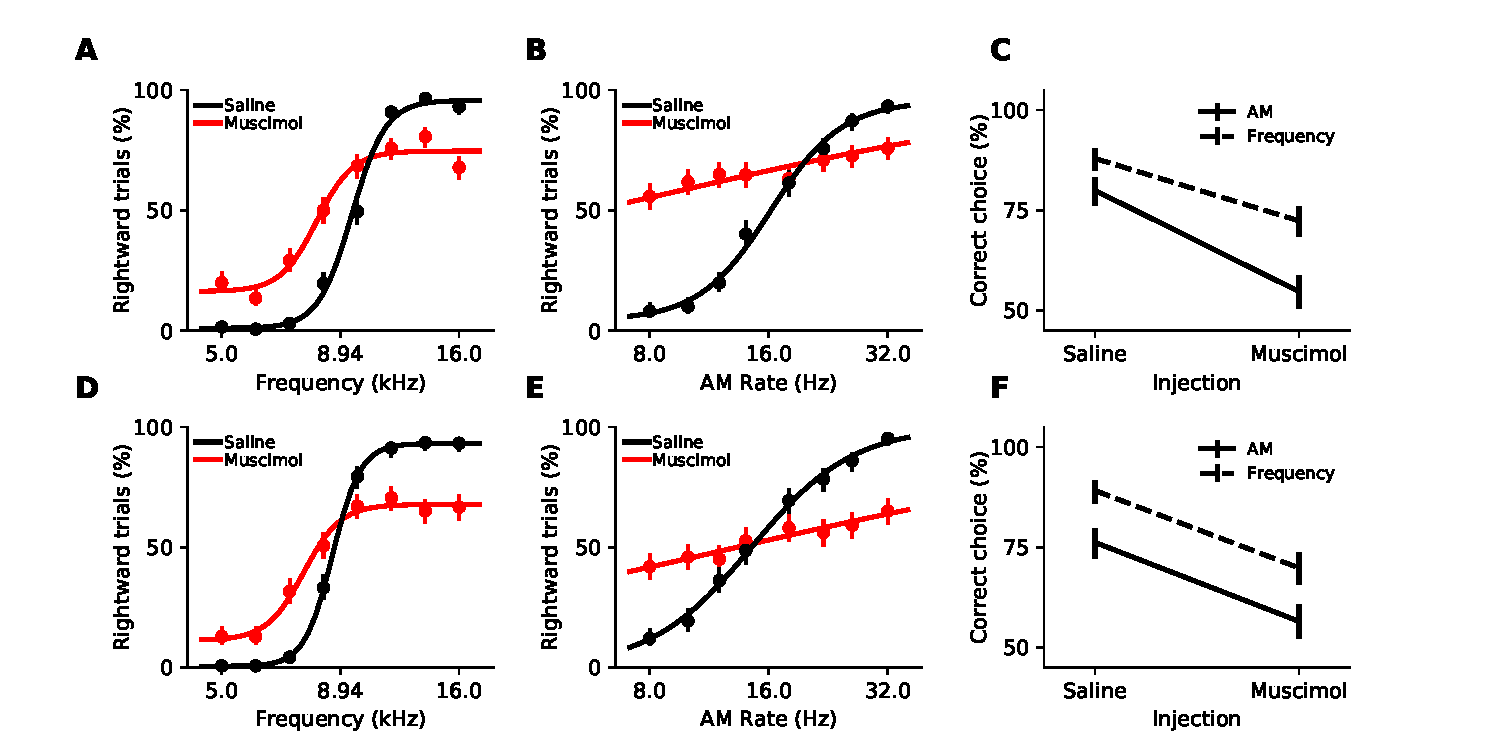
\includegraphics[width=6in]{figures/chapter4/figure_main_amod_effect}%
\end{center} \caption{Reversible inactivation of AC impairs both frequency and
AM discrimination.}{ \textbf{(A)} Frequency discrimination psychometric
performance for subject 1, averaged over 5 saline sessions (black points) and 5
muscimol sessions (red points).
%
\textbf{(B)} AM discrimination psychometric performance for subject 1, averaged
over 5 saline sessions (black points) and 5 muscimol sessions (red points). 
%
\textbf{(C)} Average percent correct for subject 1, averaged over 5 saline
sessions and 5 muscimol sessions.
%
Dotted line indicates the effect of muscimol injection on sound frequency
discrimination performance. 
%
Solid line indicates the effect of muscimol injection on AM rate discrimination
performance.
%
Error bars indicate 95\% binomial proportion confidence intervals.
%
\textbf{(D, E, F)} Same as A, B, and C, respectively, for subject 2.  }
\end{figure}

% The effect of inactivation is not different between the two stimuli (GLMER
% results).

\subsection{AC inactivation affects discrimination of both features when during
sessions with a single sound type}
% TODO: Did they learn both, and then get transferred to 2? Was it the same
% between?
For a subset of animals, we performed reversible inactivation of AC during
sessions where subjects only had to discriminate a single sound type.
%
Under these conditions, we still observed an effect of muscimol both on
psychometric performance (\textbf{\fig{\SinglePsy}}) and on overall percent
correct (\textbf{\fig{\SingleSum}}).

% We have a few sessions where we show that both discriminations are hurt
% individually, arguing against the idea that the cortically-dependent part of
% the task is the switching. 

%%%%%%%%%%%%%%%%%%%%%%%% Figure Single Sound Type %%%%%%%%%%%%%%%%%%%%%%%%%%%%%
\begin{figure}[hp] \begin{center}
	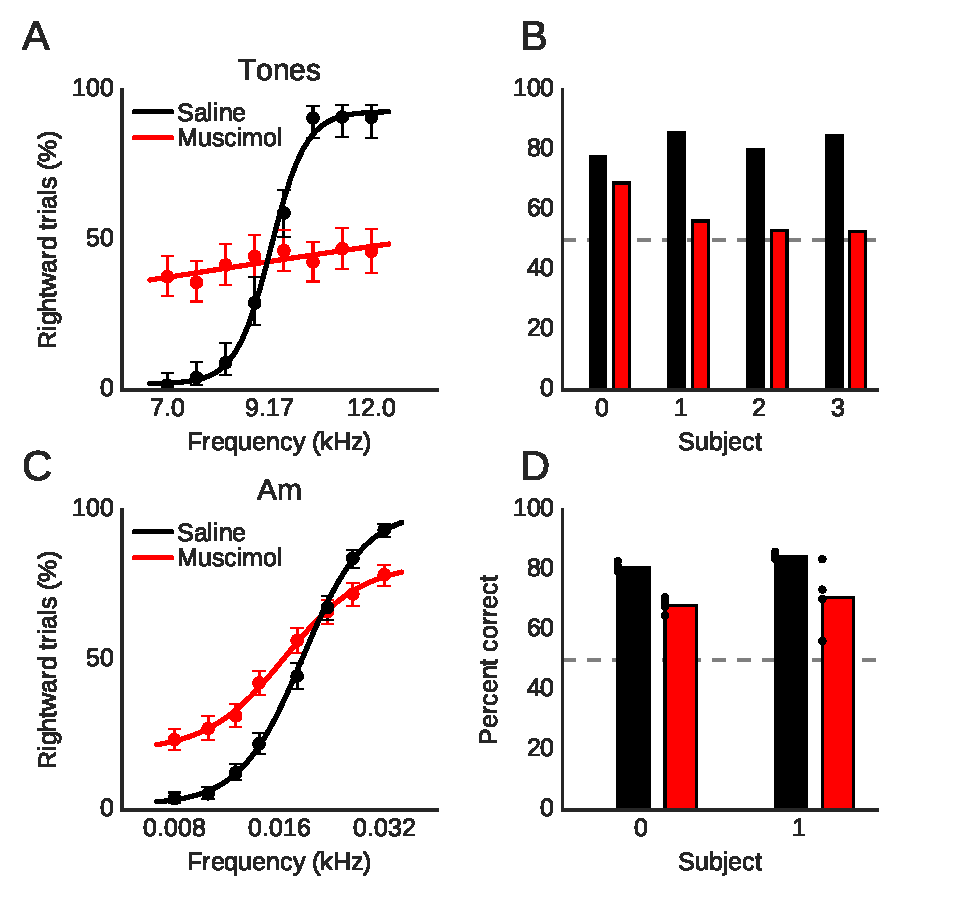
\includegraphics[width=6in]{figures/chapter4/figure_single_sound_type}%
\end{center} \caption{Muscimol affects each discrimination when performed
independently.}{\textbf{(A)}  Example psychometric curve from sessions where an
animal discriminated only high sound frequency from low sound frequency.
Performance suffers in sessions where muscimol was injected in AC (red, 1
session) compared to control saline injection (black, 1 session).
% TODO: How to have number of sessions here? 
%
\textbf{(B)} Average percent correct for 4 animals during muscimol (red, 1
session per animal) and saline (black, 1 session per animal) sessions. 
%
\textbf{(C)} Example psychometric curve from sessions where an animal
discriminated only fast AM rates from slow AM rates. Performance suffers in
sessions where muscimol was injected in AC (red, 4 sessions) compared to
control saline injection (black, 4 sessions).
%
\textbf{(D)} Average percent correct for 2 animals during muscimol (red, 4
sessions per animal) and saline (black, 4 sessions per animal) sessions.  }
\end{figure}


\section{Discussion}

In this chapter, I present a behavioral paradigm that can be used to evaluate
the effects of reversible chemical inactivation of a brain area on
discrimination of different stimuli. 
%
Using this paradigm, I trained mice to perform discriminations both of sound
frequency and of AM rate.
%
Reversible inactivation of AC with muscimol in animals trained on this task
caused deficits in discrimination of both stimuli. 
%
% It looks like the muscimol inactivation affects performance of both tasks to
% a similar degree. Several possible reasons for this: TODO: This is a bad
% sentence.
There are several possible explanations for these results. 

% TODO: Better title here
\subsection{Why did we see effects of muscimol on both frequency and AM
discrimination?}

% TODO: Write better words
%% Downstream circuits are expecting input from AC, and don't have time to complete the homeostatic rebalancing necessary to make use of information from a single source.
One reason has to do with the necessary/permissive nature of the relationship
between a brain area and a behavior \citep{Otchy2015}.
%% Less likely that the task switching component is adding an additional layer of cortical dependence, as inactivation of AC before performance of either task alone leads to performance deficits. 
An alternative explanation is that the switching component of the task
introduced an additional process that depends on the cortex, outside of the
individual sound-action associations. 
%%% Subcortical circuits can accomplish significant flexibility on a short time scale (Gimenez paper) but this is switching every trial
However, I believe that this is less likely for three reasons.

First, rodents have been shown to be capable of remarkable levels of
flexibility after nearly-complete removal of auditory cortex, switching the
action associated with a particular sound several times during a single
behavioral session \citep{Gimenez2015}.
%
%%% During training, animals learn each association independently (which takes the most time) and then learn to switch between them, which takes little time TODO: Plot this.
Second, animals took longest during the training steps in which they were
learning the individual sound-action associations, and took few trials to
achieve a high degree of accuracy after they started having to switch between
sound types in the same behavior session.
%%% Deficits caused by cortical inactivation also appear during individual AM or freq discrimination sessions, so not all effect can be related to switching. 
Lastly, we tested the effect of reversible AC inactivation during sessions with
only a single sound type in a subset of animals.
%
We observed deficits in discrimination performance during sessions with only
tonal stimuli and during sessions with just AM stimuli, suggesting that the
sound-action associations themselves are impacted by cortical inactivation.
%
Nonetheless, it is worth evaluating whether the additional complexity
introduced by switching between sound types every other trial is really
required to answer our main question. 

\subsection{Why use this method if the switching might complicate things?}

% This method took a long time to learn and there is a chance that the
% switching component introduced additional complexity.
%
% So do we need to use the task? Why is this better than the alternatives? 
This task required mice to learn two different sound-action associations, and
then to switch back and forth between them every other trial of a behavior
session.
%
Though this method presents the obvious drawbacks of taking a long time to
learn and potentially engaging additional brain areas to mediate the switching,
it allows us to evaluate the effect of a single manipulation of brain activity
on both discrimination behaviors, which is critical to addressing our main
question.

% Attempts to evaluate the effect of reversible inactivations on several
% different discriminations are hampered by the time course of the
% inactivation, and the fact that a bolus delivered on one day may not reach
% the exact same tissue area as a bolus delivered the next day.
Attempts to compare the effect of inactivations on task performance in two
different groups of animals performing the same task would invariably be
hampered by the inability to tell precisely the extent and strength of the
inactivation across individuals.
%
Even optogenetics, as will be discussed below, cannot fully address this
problem, especially if we desire to compare the size of the effect on the two
different task types.

% Problems addressed by this method:

%% Hard to compare relative effects of inactivations on different tasks across animals (one task per animal)
%%% Lesions: Have to compare lesion area across animals
%%% Muscimol: Have to compare bolus between animals, which may be impossible (except maybe with fluorescent muscimol).
%%% Optogenetics: Have to try and compare inactivated area between animals, which may be impossible. TODO: Paper Ben K presented about photobleaching relevant here.

%% Many problems still persist if you have an animal perform both tasks, but not on the same day
%%% Lesions: Time course of homeostatic rebalancing may interfere if different tasks are performed sequentially over days
%%% Muscimol: A bolus one day is not directly equivalent to a bolus the next, and fluorescent muscimol can't help you at all with that. 
%%% Optogenetics: This is less of an issue for opto, where the effects of the laser should be roughly consistent from day to day. TODO: Anything about glia growth around fibers?

%% Having animals perform both tasks during the same behavior session addresses some of these sources of variation.
%%% Lesions: Circuit rebalancing should be occurring at roughly the same pace and affecting both discriminations across assessment days.
%%% Muscimol: The effect of a single bolus can be evaluated on both tasks.
%%% Optogenetics: The state of the fiber, tether, diode, etc. that may vary from session to session are more controlled across the two tasks. 

\subsection{Are chemical inactivations useful in a world with optogenetics?}
% This is still an open question in my mind.

% TODO: Why use muscimol at all?? The problem that we are addressing with this
% interleaved task is that the inactivation wears off. This isn't as much of a
% problem with lesions, although there is still the possibility that downstream
% circuits are adapting to the changes, and so sampling different tasks on
% different days could still be a problem.

% Comparisons of lesions and optogenetics TODO: There is a paper doing visual
% cortex opto that argues against lesions.
%% Lesions: Allow time for downstream circuits to rebalance their inputs, potentially underestimating the contribution of other pathways.
%% Optogenetics: Near-instantaneous inactivation provides no chance for downstream circuits to rebalance, potentially overestimating the contribution of an area.
%% Muscimol: The worst of both worlds or better than both? Muscimol is like CNO (TODO: check arguments for CNO) but affects everything, not just HM4+ neurons, and may be stronger than HM4 inactivation (TODO: Check HM4 vs. muscimol inactivation strength). Also, there is some evidence that CNO decomposes to clozapine and becomes active elsewhere besides just at the HM4 receptors (TODO: Check new CNO to clozapine study).

% TODO: Future improvements to the task include better initial performance
% matching

Lesion studies have long been the gold standard method for evaluating the
%
A potential confound of lesions studies is often discussed: That during the
time after the lesion, subcortical pathways reorganize to carry out the
function that was previously provided by the cortex.
%
This confound rightly prevents us from inferring that cortex \emph{does not}
play a role in some particular task, if it is found that an animal is able to
perform the task after a lesion of the cortex.
%
However, with emerging anatomical studies showing extensive convergence of
cortical and thalamic pathways onto structures like the striatum
\citep{Hunnicutt2016} it is likely that both the cortical and subcortical
pathways are providing information to downstream regions during normal
conditions.
%
The re-organization of subcortical pathways following cortical lesion could
simply be a homeostatic rebalancing of already-existing connections between the
subcortical pathway neurons and the downstream region.
%
In this context, we should interpret the persistence of a behavior after
cortical lesion to mean that the cortex wasn't providing necessary information
for that behavior, not that it wasn't involved at all.

% TODO: Cite otchy and whatever paper was doing orientation change detection
% suppression in rats (Glickfeld and Maunsell)
Studies have repeatedly shown that fast, reversible inactivations (such as
those achieved with muscimol or various optogenetic methods) can lead to
different effects on the same behavior than are caused by lesions. 
%
% TODO: Getting harder to write here. Come back to this. 

Chemical inactivations complement lesions in the sense that they allow you to
test whether an area is providing information to downstream circuits under
normal conditions.
%
% TODO: this is shit and needs citations
Optogenetics is fancy and all, but has a few problems.
%
1: You can't really leave the light on forever and expect things to work as
planned.
%
2. Fast time-scale manipulations can cause local network effects and mess with
feedback inhibition and excitation, potentially messing everything up.
%
Chemical inactivations allow the brain area to reach a new steady-state that
will persist for roughly the length of time that the animal is performing the
behavior.
%
It might be possible to leave the light on if using cheeta or some other opsin
that doesn't get weaker over time, but you run the risk of frying the brain.
%
Chemical inactivations don't have that issue. 
